%%% Local Variables:
%%% TeX-command-extra-options: "-shell-escape"
%%% mode: latex
%%% TeX-master: t
%%% End:
\documentclass{beamer}
\usepackage{caption}
\usepackage{minted}
\usepackage{tikz}
\usepackage{xcolor}
\usetikzlibrary{shapes.geometric, arrows}
\tikzstyle{startstop} = [rectangle, rounded corners, minimum width=3cm, minimum height=1cm,text centered, draw=black, fill=red!30]
\tikzstyle{io} = [trapezium, trapezium left angle=70, trapezium right angle=110, minimum width=1.5cm, minimum height=0.6cm, text centered, draw=black, fill=blue!30]
\tikzstyle{process} = [rectangle, minimum width=1.5cm, minimum height=0.5cm, text centered, draw=black, fill=orange!30]
\tikzstyle{decision} = [circle, radius=2.5cm, text centered, draw=black, fill=green!30]
\tikzstyle{arrow} = [thick,->,>=stealth]
\usepackage[labelformat=simple]{subcaption}

\usetheme{Singapore}
\title{Program Design}
%\subtitle{in Racket}
%\author{Peter Campora}
%\institute{ULL}
%\date{\today}

%This lectures introduces the fundamentals of design
\begin{document}
\begin{frame}
\titlepage
\end{frame}

\begin{frame}
  ``Let's talk about design\\
  Let's talk about programmers\\
  Let's talk about code\\
  Let's talk about bugs\\
  Let's talk about design''\\\\
  -Celine Dion\\
  --Peter Campora
\end{frame}

\begin{frame}
  \frametitle{Why Does Code Quality Matter?}
  \large If the program works, who cares...\\\\
  \pause
  \huge \textbf{People will read your code later!}\\\\
  \pause
  \large Ever heard of the Y2K problem? In the 20th century, 2 digits were used to represent years...
  \begin{itemize}
  \item<4->  So, when the 21st century came, the years 1900 and 2000 would be handled identically.
  \item<5-> A ton of applications had to be updated to avoid bugs. Consider if dates were still stored in poorly named int variables.
  \item<6-> Well documented code makes such refactorings easier.
  \end{itemize}
\end{frame}

\begin{frame}
  \frametitle{It Starts With a D}
  \large What is the thing that most determines the structure of a program?\\\\
  \pause
  \begin{center}
    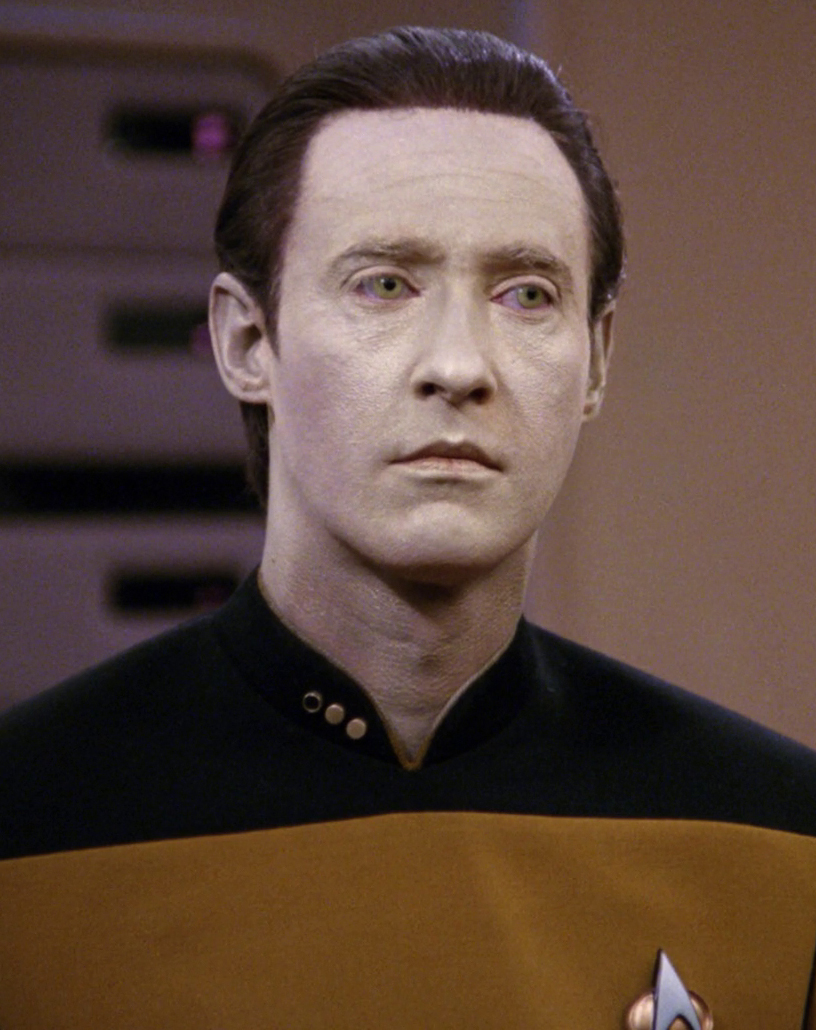
\includegraphics[width=0.4\textwidth]{images/data.jpg}
  \end{center}
\end{frame}

\begin{frame}
  \frametitle{Domains and Data}
  The two d's of software development are domains and data.
  \begin{itemize}
  \item<2-> The quantity, 5, means different things in different \emph{domains}. For a game, 4 might be the number of pixels an object should move per clock tick. For furniture website, 4 might represent the number of legs on a chair.
  \item<3-> Information in English is usually given to programmers to indicate the structure of the domain. Our job is to turn this information into \emph{data}
    representations. 
  \item<4-> After we have data representations for our domain, a program becomes a matter of data transformation.
  \item<5-> The final data produced by the program is some sort of information about our domain.
  \item<6-> If the final data is 42, this might be some height in pixels, the number of units sold, the meaning of life...etc.
  \end{itemize}
\end{frame}

\defverbatim[colored]\dataDef{
\begin{minted}{racket}
  ; A Temperature is a Number. 
  ; interpretation represents Celsius degrees
\end{minted}
}

\begin{frame}
  \frametitle{Data Interpretation}
  For now, we will specify the interpretation of data in comments (later we will define data types).
  \begin{itemize}
  \item<2-> We will call these data definitions. 
  \item<3-> Here's an example: \dataDef
  \item<4-> This specifies that the numbers produced by our program (or function) represent Celsius degrees
  \item<5-> Such a specification rules out ``cold'' as a temperature but not -400 (which is not a real C temp)
  \item<6-> Later, we will learn to put such specifications on data, but for now our english descriptions suffice
  \end{itemize}
\end{frame}

\begin{frame}
  \frametitle{The Design Process}
  Keeping Data Interpretation in mind, let's turn to our program design process.
  \begin{enumerate}
  \item<2-> Express how you wish to represent information as data. A one-line comment for specifying \emph{data interpretations} suffices.
  \item<3-> Write down a signature, a statement of purpose, and a function header.
    \begin{itemize}
    \item<4-> A \emph{signature} communicates the domain and codomain of your function. For example: \mintinline{racket}{; Number Number -> Number}
    \item<5-> A \emph{statement of purpose} communicates what the function produces and how it produces the answer
    \item<6-> A \emph{function header} is merely a stub definition for the function with a name, parameters, and a trivial body: \mintinline{racket}{(define (add x y) 0)}
    \end{itemize}    
  \end{enumerate}
\end{frame}

\defverbatim[colored]\squareExample{
\begin{minted}{racket}
    ; Number -> Number
    ; computes the area of a square with side len 
    ; given: 2, expect: 4
    ; given: 7, expect: 49
    (define (area-of-square len) 0)
\end{minted}
}

\defverbatim[colored]\squareTests{
\begin{minted}{racket}
    (sqr 2); gives: 4
    (sqr 7); gives: 49
\end{minted}
}

\begin{frame}
  \frametitle{The Design Process (cont.)}
  \begin{enumerate}
    \setcounter{enumi}{2}
  \item Create \emph{functional examples} that illustrate the expected input and output behaviors of a function. Consider a function that computes the square of a number: \squareExample
  \item<2-> \emph{Take inventory} for the program. See what is given and what needs to be computed. Basically, each function header indicates
    what is needed and then we start to skeleton the body based on the parameters:
    \begin{itemize}
    \item<3-> \mintinline{racket}{(define (area-of-square len) (... len ...))}
    \item<4-> The dots indicate where the function needs to be fleshed out.    
    \end{itemize}
  \end{enumerate}
\end{frame}

\begin{frame}
  \frametitle{The Design Process (cont.)}
  \begin{enumerate}
    \setcounter{enumi}{4}
  \item<2-> Now we finally \emph{code}. Based on our inventory and functional examples, we should have some idea of what to replace the ... with.
    For the program we've been discussing, our function body becomes \mintinline{racket}{(sqr len)}, where the second ... is removed.
  \item<3-> The final step is \emph{testing} the definition based on our functional examples.
    We'll first verify the correctness of this definition in Racket. But if we made a mistake it could be one of three kinds:
    \begin{itemize}
    \item<4-> (1) The functional examples were wrong.
    \item<5-> (2) The function definition was wrong and needs to be rewritten.
    \item<6-> (3) Both the examples and the definition were wrong.
    \item<7-> In any case, we have to back and verify that steps 3 was done correctly, and if it was, then we head back to step 5. Otherwise, fix the examples and retest.
    \end{itemize}    
  \end{enumerate}
\end{frame}

% \begin{frame}
%   \frametitle{Homework 2}
%   For our second homework, I want you to repeat writing certain functions from the first homework but using the
%   design process.
%   \begin{enumerate}
%   \item Design the function string-first, which extracts the first character from a non-empty string. Don’t worry about empty strings.
%   \item Design the function string-last, which extracts the last character from a non-empty string.
%   \item Design the function image-area, which counts the number of pixels in a given image.
%   \item Design the function string-rest, which produces a string like the given one with the first character removed.
%   \item Design the function string-remove-last, which produces a string like the given one with the last character removed. 
%   \end{enumerate}
% \end{frame}


\begin{frame}
  \frametitle{Programming in Different Domains}
  There are two different kinds of domain knowledge that programmers typically deal with.
  \begin{enumerate}
  \item<2-> One is knowledge from external domains. In Lafayette alone, there are programmers working on programs dealing with pharmaceutical operations, food  delivery, ambulance services, jewelry, oil field technology, insurance claims, and more. So  how do programmers figure out how to write functions
    for dealing with these different domains? One necessary skill is to learn math, which is common to many domains. The other is to learn communication skills so that you can pick up necessary skills for new domains by communicating with experts in these fields.
  \item<3-> The other domain knowledge that is used is knowledge of library functions. Knowing what things are already written for you greatly speeds up development.
    Don't reinvent the wheel.
  \end{enumerate}  
\end{frame}

\begin{frame}
  \frametitle{From Functions to Programs}
  It's rare that a program consists of a single function definition unless it's trivial or poorly written. So why does the need for multiple functions arise?
  \begin{itemize}
  \item<2-> When designing an interactive program, we need separate functions for handling different events, like handling a mouse click versus a keyboard press.
  \item<3-> For batch programs, auxiliarly functions are needed when solving some subpart of the overall problem. For example, we need a function to square numbers
    when defining a batch program that computes the area of a circle when given its radius and the area of a square when given a side length.
  \item<4-> Although not a necessity, often we encounter that the same computation is needed twice, and copying code is tedious and error-prone.
  \item<5-> For these reasons for needing functions, programmers should keep a \emph{wish list} of functions that they need to define.
  \end{itemize}
  
\end{frame}

\begin{frame}
  \frametitle{Wish Lists}
  \begin{center}
    \includegraphics[width=0.25\textwidth]{images/christmas-list.jpeg}
  \end{center}
  \begin{itemize}
  \item<2-> Here's an algorithm for writing programs with a wish list.
  \item<3-> If writing a batch program, put the main function on the list. If writing an interactive program, put the event handling functions, etc. on the wish list.
  \item<4-> Take an item off of the wish list and start designing it.
  \item<5-> When designing the function, if it seems that another function is necessary to finish the current design, then put this new function on the wish list and
    start designing it.
  \item<6-> Keep designing functions on the wish list until no more remain. After this, the program should be complete.
  \end{itemize}
\end{frame}

\begin{frame}
  \frametitle{Everyone's Favorite Activity}
  \begin{center}
    \includegraphics[width=0.4\textwidth]{images/testing.png}
  \end{center}
  \begin{itemize}
  \item<2-> Love it or hate it, testing is an essential part of software development, as we want our software to behave correctly and predictably. 
  \item<3-> Testing functions by loading the program and using the repl with manual input values is a tedious and brittle way to ensure the validity of programs.
  \item<4-> So, we want a facility to mechanize testing, which Racket (and most languages) provides.
  \item<5-> What are we waiting for? Let's get cooking (testing)!
  \end{itemize}
\end{frame}

\defverbatim[colored]\testProgram{
\begin{minted}{racket}
  ; Number -> Number 
  ; converts Fahrenheit temperatures to Celsius
  ; given 32, expect 0
  ; given 212, expect 100
  ; given -40, expect -40
  (define (f2c f)
    (* 5/9 (- f 32)))
\end{minted}
}

\defverbatim[colored]\tests{
\begin{minted}{racket}
    (check-expect (f2c -40) -40)
    (check-expect (f2c 32) 0)
    (check-expect (f2c 212) 100)
\end{minted}
}

\begin{frame}
  \frametitle{Check Your Expectations}
  Let us consider testing a Fahrenheit to Celsius conversion program:
  \testProgram
  \begin{itemize}
  \item<2-> Our tests should be created from our functional examples.
  \item<3-> Using rackets \mintinline{racket}{check-expect} form, we can write the appropriate tests:
    \tests
  \end{itemize}
\end{frame}

\begin{frame}
  \frametitle{Testing (cont.)}
  \begin{itemize}
  \item  The general expression \mintinline{racket}{(check-expect exp-to-test expected-value)} says that the expression \mintinline{racket}{exp-to-test}
    should evaluate to \mintinline{racket}{expected-value}, and otherwise the test fails.
  \item<2-> To run tests under Racket, we add the expression \mintinline{racket}{(test)} to our file.
  \item<3-> You can add test expressions before a function is even defined, and it will be fine.
  \item<4-> You can also test images in Dr Racket:
    \includegraphics[width=0.4\textwidth]{images/test-image.png}
  \item<5-> Write lots of tests so that you can be confident in the correctness of your programs as you develop them!
  \end{itemize}
\end{frame}

\begin{frame}
  \frametitle{Interactive Program Love}
  These lectures will focus more on interactive programs for a while.
  \begin{center}
    \includegraphics[width=0.7\textwidth]{images/dan-arin-matt.png}
  \end{center}
\end{frame}

\begin{frame}
  \frametitle{How to Design Interactive Programs}
  Our previous discussion of event-driven bigbang programs was done in an ad hoc way. Now we discuss how to systematically design such programs.
  \begin{itemize}
  \item<2-> To start designing world programs, you must first create a data definition for all possible states.
  \item<3-> Then comes writing stubs for each of the event handling functions.
  \item<4-> Then the stubs for the exit and rendering functions.
  \item<5-> Putting these all together creates our wish list.
  \end{itemize}
\end{frame}

\begin{frame}
  \frametitle{An Example Wish List}
  \begin{center}
    \includegraphics[width=0.7\textwidth]{images/wish-list.png}
  \end{center}
\end{frame}

\defverbatim[colored]\constants{
\begin{minted}{racket}
    (define WIDTH-OF-WORLD 200) ;physical constant
    ...
    (define WHEEL
      (circle WHEEL-RADIUS "solid" "black")) ;graphical constant
\end{minted}
}

\defverbatim[colored]\worldState{
\begin{minted}{racket}
      ; A WorldState is a Number.
      ; interpretation the number of pixels between
      ; the left border of the scene and the car
\end{minted}
}

\begin{frame}
  \frametitle{Interactive Design By Example}
  Let's illustrate the rest of the design for an interactive program by example.
  We will have three big steps to illustrate and one small one.
  \begin{itemize}
  \item<2-> Let's animate a car moving across the screen, moving to the right 3 pixels per clock tick. 
  \end{itemize}
  \begin{enumerate}
  \item<3-> For all properties of the world that do not change, introduce constants.
    We will introduce constants for the description for the car. These are separated into two parts, graphical and physical constants:
    \constants
  \end{enumerate}
\end{frame}

\begin{frame}
  \frametitle{Interactive Design By Example (cont.)}
  \begin{enumerate}
    \setcounter{enumi}{1}
  \item<1-> Other properties do change over time and events and determine the state of the world. We must give an interpretation of what our world state means.
    \begin{itemize}
    \item<2-> So, based on our problem description what changes over time?
    \item<3-> Right, so our worldState is the position of the car:
      \worldState
    \end{itemize}
  \item<4-> After defining constants and the interpretation of our world state,
    we can start defining the relevant functions that will be on our wish list.
    \begin{itemize}
    \item<5-> Typically our wish list starts with our event handling functions, something to indicate when the program terminates, and our render function
    \item<6-> For this program, there is only 1 event that we need to handle. What is it?
    \end{itemize}
  \end{enumerate}
\end{frame}

\defverbatim[colored]\tock{
\begin{minted}{racket}
  ; WorldState -> WorldState
  ; adds 3 to x to move the car right 
  (define (tock x) x)
\end{minted}
}

\defverbatim[colored]\render{
\begin{minted}{racket}
  ; WorldState -> Image
  ; places the image of the car x pixels from 
  ; the left margin of the BACKGROUND image 
  (define (render x) BACKGROUND)
\end{minted}
}

\begin{frame}
  \frametitle{Interactive Design By Example (cont.)}
  Since the problem description doesn't specify anything about user
  input, we only have to handle clock events. Moreover, we don't have a specification that the car should stop at the right edge of the screen, so no termination function is needed. So what functions are on our wishlist that we need to apply our design process to?
  \begin{enumerate}
  \item<2-> We need a function \mintinline{racket}{tock} for handling clock ticks
  \item<3-> We need a function \mintinline{racket}{render} to draw the scene.
  \end{enumerate}
  \begin{itemize}
  \item<4-> Skeletoning out our tock function:
    \tock
  \item<5-> Our render function:
    \render
  \end{itemize}
\end{frame}

\defverbatim[colored]\mainProg{
\begin{minted}{racket}
; WorldState -> WorldState
; launches the program from some initial state 
(define (main ws)
   (big-bang ws
     [on-tick tock]
     [to-draw render]))
\end{minted}
}

\begin{frame}
  \frametitle{Interactive Design By Example (cont.)}
  For our final step we need to design our main function that makes
  use of our tock and render functions. The structure of main is
  straightforward from the rest of the process so far. 
  \begin{itemize}
  \item<2-> \mainProg
  \item<3-> And that's it for skeletoning out this example! First, define constants,
    second give a world state interpretation, third start defining relevant
    functions on the wishlist, and fourth define the main function as a
    big bang expression. Now we use the design process for functions to finish
    the definitions for tock and render.
  \end{itemize}
\end{frame}

\defverbatim[colored]\tockSkeleton{
\begin{minted}{racket}
  ;   given: 20, expect 23
  ;   given: 78, expect 81
  (define (tock ws) (... ws ...))
\end{minted}
}

\begin{frame}
  \frametitle{Interactive Design By Example (cont.)}
  Using step 4 of our design process for functions, let us give input
  and output examples for our tock function. and skeleton out the rest of the body.
  \begin{itemize}
  \item<2-> \tockSkeleton
  \item<3-> After this, we finish the body of the function as
    \mintinline{racket}{(define (tock ws) (+ ws 3))}
  \item<4-> Finally, we can add tests to verify the correctness of the function:
    \mintinline{racket}{(check-expect (tock 20) 23)} and \mintinline{racket}{(check-expect (tock 78) 81)}.
  \item<5-> And similarly we can use our process to finish the render function.
    For now, we move on to making an interesting modification to the program.
  \end{itemize}  
\end{frame}

\defverbatim[colored]\moveCar{
\begin{minted}[fontsize=\footnotesize]{racket}
  ; Number Number Number String -> Number
  ; If the mouse event is a click down,
  ; move the x-coordinate of the world state
  ; Given: 30 10 20 "button-down" Expect: 10
  ; Given: 30 10 20 "enter" Expect: 30
  ; Given: 30 10 20 "move" Expect: 30
  (define (move-car car-position x-click y-click click-kind) ...)
\end{minted}
}

\begin{frame}
  \frametitle{Real Interaction}
  Let's modify our car program so that a car can teleport to where a user clicks
  on the canvas (the x-coordinate, y won't change).
  \begin{itemize}
  \item<2-> What will we need to add to our big-bang expression to handle this
    new criteria?
  \item<3-> Right, we need to add a function for the on-click handler.
  \item<4-> But what arguments will click events pass to our function?
  \item<5-> It passes the x-coordinate, y-coordinate, and whether or not the
    mouse clicked down, was released, or was moved.
  \item<6-> So, we need something like:
    \moveCar
  \end{itemize}
\end{frame}

\defverbatim[colored]\moveCar{
\begin{minted}[fontsize=\footnotesize]{racket}
  (define (move-car car-position x-click y-click click-kind) 
    (cond
      [(string=? click-kind "button-down") x-click]
      [else car-position]))
\end{minted}
}

\begin{frame}
  \frametitle{Real Interaction (cont.)}
  Based on our functional examples, the body of move-car needs to be a
  conditional expression that depends on the string given:
  \begin{itemize}
  \item<2-> \moveCar
  \item<3-> Then the last thing we need to do is add:
    \mintinline{racket}{[on-click move-car]} to the big-bang expression.
  \item<4-> So, our modifications to this program was relatively simple. Why?
    Two reasons:
    \begin{enumerate}
    \item<5-> Our program is separated into a \emph{model} that represents
      the position of the car and the state of the world and a \emph{view}
      that renders the scene based on the model.
    \item<6-> The design recipes clearly relate a change in the problem description
      to an event that needs to be handled.
    \end{enumerate}
  \end{itemize}
\end{frame}

\defverbatim[colored]\mouseEnum{
\begin{minted}{racket}
  ; A MouseEvt is one of these Strings:
  ; – "button-down"
  ; – "button-up"
  ; – "drag"
  ; – "move"
  ; – "enter"
  ; – "leave"
\end{minted}
}

\begin{frame}
  \frametitle{Intervals, Enumerations, and Itemizations}
  So far our programs haven't had a lot of different states that they could
  be in that complicate the conditional logic of the program.
  \begin{itemize}
  \item<2-> We've already discussed \mintinline{racket}{cond} expressions.
  \item<3-> Now we will consider \emph{enumerations} which represent the alternative states our data can be in.
  \item<4-> Remember in previous programs that we have to inspect strings
    to discover if the correct mouse or key event happened
  \item<5-> \mouseEnum
  \end{itemize}
\end{frame}

\defverbatim[colored]\trafficEnum{
\begin{minted}{racket}
  ; A TrafficLight is one of the following Strings:
  ; – "red"
  ; – "green"
  ; – "yellow"
  ; interpretation the three strings represent the three 
  ; possible states that a traffic light may assume 
\end{minted}
}

\begin{frame}
  \frametitle{Enumerations}
  We sometimes need to define our own enumerations to describe
  the state of our application. For example, we can describe
  the state of a traffic light as follows:
  \begin{itemize}
  \item<2-> \trafficEnum
  \item<3-> So, let's say that now we want a program to animate the changing
    of a traffic light, starting from a red light
  \item<4-> Although I'm pretty sure we all know how traffic lights transition,
    I'll draw a state machine on the board.
  \item<5-> How does this state machine translate to code?    
  \end{itemize}
\end{frame}

\defverbatim[colored]\trafficTransition{
\begin{minted}{racket}
  ; TrafficLight -> TrafficLight
  ; yields the next state given current state s
  (check-expect (traffic-light-next "red") "green")
  (define (traffic-light-next s)
    (cond
      [(string=? "red" s) "green"]
      [(string=? "green" s) "yellow"]
      [(string=? "yellow" s) "red"]))
\end{minted}
}

\begin{frame}
  \frametitle{Enumerations (cont.)}
  The conditional nature of state and transitions in a state machine
  directly translate to a function with a conditional expression.
  \begin{itemize}
  \item<2-> \trafficTransition
  \item<3-> We should probably add more tests to verify that our definition
    works, but we will skip this for now.
  \item<4-> Homework: Write a big bang program to animate a continuous
    traffic light transition sequence (don't worry if it flashes through the
    colors far too rapidly).
  \end{itemize}
\end{frame}

\defverbatim[colored]\keyEnum{
\begin{minted}{racket}
  ; A KeyEvent is one of: 
  ; – 1String
  ; – "left"
  ; – "right"
  ; – "up"
  ; – ...
\end{minted}
}



\begin{frame}
  \frametitle{Enumerations (cont.)}
  An important thing about enumerations to remember is that there are
  only a finite amount of alternatives to consider. 
  \begin{itemize}
  \item<2-> The bad thing about our approach so far is that
    we have to specify our data alternatives in comments and then
    when encountering a function taking an enumeration as input, we
    write a cond expression handling each alternative.
  \item<3-> Consider key events as an enumeration:
    \keyEnum
  \end{itemize}
\end{frame}

\defverbatim[colored]\keHandler{
\begin{minted}{racket}
  ; WorldState KeyEvent -> ...
  (define (handle-key-events w ke)
    (cond
      [(= (string-length ke) 1) ...]
      [(string=? "left" ke) ...]
      [(string=? "right" ke) ...]
      [(string=? "up" ke) ...]
      [(string=? "down" ke) ...]
      ...))
\end{minted}
}

\begin{frame}
  \frametitle{Handling Enumerations Systematically}
  The specification of our enumeration \emph{directly} gives rise
  to the structure of our handler.
  \begin{itemize}
  \item<2-> Cond handles each key input:
    \keHandler
  \item<3-> It's like \emph{algebra}. If you need to solve a quadratic
    equation, use the quadratic formula...
  \item<4-> If data is represented as an enumeration, write a function
    that matches against the alternatives of the enumeration.
  \end{itemize}
\end{frame}

\begin{frame}
  \frametitle{Enumerations By Example}
  It's pretty common that we only have to consider a subset of the
  overall set of possible enumerations for some state. Let's illustrate
  this by considering a program that only uses a subset of the key events:
  \begin{itemize}
  \item<2-> Design a key-event handler that moves a red dot left or right on a horizontal line in response to pressing the left and right arrow keys.
  \item<3-> We must differentiate the left and right arrow keys from
    other key presses.
  \item<4-> Let's employ our design process!
  \end{itemize}
\end{frame}

\defverbatim[colored]\keInterp{
\begin{minted}[fontsize=\footnotesize]{racket}
  ;; A Position is a natural number
  ;; whose interpretation measures distance from the left axis.  
\end{minted}
}

\defverbatim[colored]\keHeader{
\begin{minted}{racket}
  ; Position KeyEvent -> Position
  ; computes the next location of the ball 
  (define (key-handler position key-event) ...)
\end{minted}
}

\defverbatim[colored]\keTests{
\begin{minted}{racket}
  (check-expect (key-handler 13 "left") 8)
  (check-expect (key-handler 13 "right") 18)
  (check-expect (key-handler 13 "a") 13)
\end{minted}
}

\begin{frame}
  \frametitle{Designing a Key Handler}
  What's the first step to designing this function
  \begin{itemize}
  \item<2->That's right, design a data interpretation for our world state.
  \item<3-> \keInterp
  \item<4-> Now, we write a signature, a statement of purpose, and a 
    function header.
  \item<5-> \keHeader
  \item<6-> Now we need to give an example of some expected input and output pairs.
  \item<7-> \keTests
  \end{itemize}
\end{frame}

\defverbatim[colored]\keDef{
\begin{minted}{racket}
  (define (key-handler p k)
    (cond
      [(= (string-length k) 1)
       p]
      [(string=? "left" k)
       (- p 5)]
      [(string=? "right" k)
       (+ p 5)]
      [else p]))
\end{minted}
}

\begin{frame}
  \frametitle{Designing a Key Handler (cont.)}
  Now we can start fleshing out the definition of \mintinline{racket}{key-handler}.
  \begin{itemize}
  \item<2-> Based on our examples, and specification of
    the KeyEvent enumeration we need a cond expression.
  \item<3-> \keDef
  \end{itemize}
\end{frame}

\defverbatim[colored]\keNew{
\begin{minted}{racket}
  (define (key-handler p k)
    (cond
      [(string=? "left" k)
       (- p 5)]
      [(string=? "right" k)
       (+ p 5)]
      [else p]))
\end{minted}
}

\begin{frame}
  \frametitle{Designing a Key Handler (cont.)}
  The previous program was designed based on the idea that we
  consider each case of our enumeration and add a cond clause.
  Is there anything wrong with it?
  \mintinline{racket}{key-handler}.
  \begin{itemize}
  \item<2-> We didn't need the first clause for checking for Characters
    and can refactor it as follows:
  \item<3-> \keNew
  \item<4-> In general, we should program in such a matter, writing
    a working version first and refactoring to a cleaner definition later.
  \end{itemize}
\end{frame}

\begin{frame}
  \frametitle{Intervals and Itemizations}
  Most of you should be familiar with the idea of an interval. It is simply
  a range of numbers that should be considered, without a need for
  explicit enumeration.
  Writing conditions to deal
  with different ranges should not be difficult to you by now. So, I will
  focus more on \emph{itemizations} which generalize enumerations and intervals.
  \begin{itemize}
  \item<2-> An itemization can contain enumerations and intervals or any
    combination of data possibilities from separate domains.
  \item<3-> An example of a function whose signature uses an
    itemization is \mintinline{racket}{string->number}, with
    the signature \mintinline{racket}{String -> NorF}
  \item<4-> A \mintinline{racket}{NorF} is either \mintinline{racket}{false}
    or an element of type \mintinline{racket}{Number}
  \item<5-> Let's start writing some function that uses the \mintinline{racket}{NorF} itemization to illustrate how it's done.
  \end{itemize}
\end{frame}

\defverbatim[colored]\condAdd{
\begin{minted}{racket} 
  (cond
    [(false? x) ...]
    [else ...])
\end{minted}
}

\defverbatim[colored]\addThree{
\begin{minted}{racket}
; NorF -> Number
; adds 3 to the given number; 3 otherwise
(check-expect (add3 #false) 3)
(check-expect (add3 0.12) 3.12)
(define (add3 x)
  (cond
    [(false? x) 3]
    [else (+ x 3)]))
\end{minted}
}

\begin{frame}
  \frametitle{Using Itemizations}
  Let's consider writing a program that adds three to an input
  of type \mintinline{racket}{NorF}. It should treat \mintinline{racket}{false}
  as 0, similar to many languages (like Python).
  \begin{itemize}
  \item<2-> What does my signature look like?
  \item<3-> \mintinline{racket}{; NorF -> Number}
  \item<4-> What should we replace ''...'' with in this test?
    \mintinline{racket}{(check-expect (add3 false) ...)}
  \item<5-> \mintinline{racket}{(check-expect (add3 false) 3)}
  \item<6-> A test for checking numbers is straightforward:
    \mintinline{racket}{(check-expect (add3 0.12) 3.12)}
  \item<7-> The body of our function will have to check what the type
    of the data we received is:
  \item<8-> \condAdd
  \end{itemize}
\end{frame}

\begin{frame}
  \frametitle{Using Itemizations (cont.)}
  It should be straightforward to define the rest of the program after this:
  \pause
  \addThree
  \pause
  There's something a bit deeper going on with Itemizations that we'll
  get into later...but for now we should just write more programs!
\end{frame}

\defverbatim[colored]\LRCD{
\begin{minted}{racket}
    ; An LRCD (for launching rocket countdown) is one of:
    ; – "resting"
    ; – a Number between -3 and -1
    ; – a NonnegativeNumber 
    ; interpretation a grounded rocket, in countdown mode,
    ; a number denotes the number of pixels between the
    ; top of the canvas and the rocket (its height)
\end{minted}
}

\defverbatim[colored]\rocketConstants{
\begin{minted}[fontsize=\footnotesize]{racket}
    (define SCENE-HEIGHT 300) ; distances in pixels 
    (define SCENE-WIDTH  100)
    (define YDELTA 3)
 
    (define BACKGROUND  (empty-scene SCENE-WIDTH SCENE-HEIGHT))
    (define ROCKET (rectangle 5 30 "solid" "red"))
 
    (define CENTER (/ (image-height ROCKET) 2))
\end{minted}
}

\begin{frame}
  \frametitle{Return to NASA}
  Let's write a program to launch a Rocket with a countdown!
  The countdown starts when the space bar is pressed and counts down from
  3. After reaching 0, liftoff is achieved and the rocket flies 3 pixels
  per clock tick upwards.
  \begin{itemize}
  \item<2-> This program is more involved than previous ones we wrote.
  \item<3-> Let us start by following our program design recipe and
    defining our global constants.
  \item<4-> \rocketConstants
  \item<5-> Our next step is to give our data interpretation for the program,
    which is more involved.
  \end{itemize}
\end{frame}

\defverbatim[colored]\rocketWish{
\begin{minted}[fontsize=\footnotesize]{racket}
  ; LRCD -> Image
  ; renders the state as a resting or flying rocket 
  (define (show x)
    BACKGROUND)
 
  ; LRCD KeyEvent -> LRCD
  ; starts the countdown when space bar is pressed, 
  ; if the rocket is still resting 
  (define (launch x ke)
    x)
 
  ; LRCD -> LRCD
  ; raises the rocket by YDELTA,
  ;  if it is moving already 
  (define (fly x)
    x)
\end{minted}
}

\defverbatim[colored]\showTestOne{
\begin{minted}{racket}
  (check-expect (show "resting")
    (place-image ROCKET 10 SCENE-HEIGHT BACKGROUND))
\end{minted}
}

\begin{frame}
  \frametitle{Return to NASA (cont.)}
  So position is obviously part of the state, but the state
  should also indicate if the space bar has not been pressed. And we also
  need state for representing the countdown, an interval. What does this look like?
  \begin{itemize}
  \item<2-> \LRCD
  \end{itemize}  
\end{frame}

\begin{frame}
  \frametitle{Return to NASA (cont.)}
  Since this is a big-bang program, we create a wishlist of functions for
  handling key presses, handling clock ticks, and rendering an image. It should
  look something like the following:
  \pause
 \rocketWish    
\end{frame}

\defverbatim[colored]\showTestTwo{
\begin{minted}[fontsize=\footnotesize]{racket}
  (check-expect
   (show -2)
   (place-image (text "-2" 20 "red")
                10 (* 3/4 WIDTH)
                (place-image ROCKET 10 SCENE-HEIGHT BACKGROUND)))
\end{minted}
}

\defverbatim[colored]\showTestThree{
\begin{minted}{racket}
  (check-expect
   (show 53)
   (place-image ROCKET 10 53 BACKGROUND))
\end{minted}
}

\begin{frame}
  \frametitle{Show the Rocket!}
  Before we start developing our rendering function, we must provide some
  functional examples.
  \begin{itemize}
  \item<2-> \showTestOne
  \item<3-> This test is straightforward, the rocket should remain at the
    bottom of the screen
  \item<4-> Let's make a test for when the countdown is happening. We will
    assume that the countdown is drawn at (10, 3/4*width).
  \item<5-> \showTestTwo
  \end{itemize}
\end{frame}

\begin{frame}
  \frametitle{Show the Rocket! (cont.)}
  We need one last test to illustrate what the rocket should do once
  it has launched.
  \begin{itemize}
  \item<2-> \showTestThree
  \item<3-> Quickly evaluating our expected results in DrRacket
    shows that our rocket is halfway into the ground...
  \item<4-> Always try to specify your tests correctly, or it
    is hard to debug programs. Let's fix our tests.
  \item<5-> These input and output examples illustrate that our
    \mintinline{racket}{show} function must have a cond expression
    handling the different types of data in our LRCD itemization.
  \end{itemize}
\end{frame}

\defverbatim[colored]\showSkeleton{
\begin{minted}{racket}
    (define (show x)
      (cond
        [(string? x) ...]
        [(<= -3 x -1) ...]
        [(>= x 0) ...]))
\end{minted}
}

\begin{frame}
  \frametitle{Show the Rocket! (cont.)}
  So, let's make a skeleton for show:
  \begin{itemize}
  \item<2-> \showSkeleton
  \item<3-> Recall that each cond clause corresponds to some part of the
    itemization, as did our tests.
  \item<4-> By looking at our first test, we can easily finish the first
    cond clause
  \item<5-> \mintinline{racket}{(place-image ROCKET 10 SCENE-HEIGHT BACKGROUND)}
  \end{itemize}
\end{frame}

\defverbatim[colored]\countDown{
\begin{minted}[fontsize=\footnotesize]{racket}
    (place-image 
      (text (number->string x) 20 "red") 10 (* 3/4 SCENE-WIDTH) 
        (place-image ROCKET 10 SCENE-HEIGHT BACKGROUND))
\end{minted}
}

\begin{frame}
  \frametitle{Show the Rocket! (cont.)}
  Now we need to finish the last two clauses. Notice that between -3 and -1,
  we want to display a  number in the countdown, and so we need some way of
  converting these values to strings.
  \begin{itemize}
  \item<2-> Anyone recall how to get a string from a number in Racket?
  \item<3-> With \mintinline{racket}{number->string}, we can now produce
    the countdown text and place the rocket at the bottom of the image.
  \item<4-> \countDown
  \item<5-> The last clause is nice and simple and places the rocket at $\mintinline{racket}{x} - \mintinline{racket}{CENTER}$ when $\mintinline{racket}{x} \ge 0$.
  \item<6-> \mintinline{racket}{(place-image ROCKET 10 (- x CENTER) BACKGROUND)}
  \end{itemize}
\end{frame}

\begin{frame}
  \frametitle{Launch!}
  Whew finishing fly took a while! And we still have two more functions
  to develop! Let's develop our key-event handling function
  \mintinline{racket}{launch} first.
  \begin{itemize}
  \item<2-> As usual let's start developing our functional examples.
  \item<3-> \mintinline{racket}{(check-expect (launch "resting" " ") -3)}
  \item<4-> \mintinline{racket}{(check-expect (launch "resting" "a") "resting")}
  \item<5-> \mintinline{racket}{(check-expect (launch -3 " ") -3)}
  \item<6-> \mintinline{racket}{(check-expect (launch 2 " ") 2)}
  \item<7-> There are more cases that we can consider, but this is enough
    for now.
  \item<8-> Similar to designing \mintinline{racket}{show}, our tests and
    used of an itemization tell us that we need a conditional expression.
  \end{itemize}
\end{frame}

\defverbatim[colored]\launchSkeleton{
\begin{minted}{racket}
    (define (launch x ke)
      (cond
        [(string? x) ...]
        [(<= -3 x -1) ...]
        [(>= x 0) ...]))
\end{minted}
}

\defverbatim[colored]\launchSimple{
\begin{minted}{racket}
    [(<= -3 x -1) x]
    [(>= x 0) x]
\end{minted}
}

\begin{frame}
  \frametitle{Launch! (cont.)}
  So, let's skeleton out our definition:
  \begin{itemize}
  \item<2-> \launchSkeleton
  \item<3-> Fleshing out the first condition based on the tests is simple:
  \item<4-> \mintinline{racket}{(if (string=? ke " ") -3 x)}
  \item<5-> The next two conditions are very simple:
    \launchSimple
  \item<6-> Filling in our skeleton with these three conditions,
    finishes the definition of \mintinline{racket}{launch}
  \end{itemize}
\end{frame}

\begin{frame}
  \frametitle{Pretty Fly for a Program}
  The last function we need to define is our clock tick handling
  function \mintinline{racket}{fly}.
  \begin{itemize}
  \item<2-> You know the drill...
  \item<3-> \mintinline{racket}{(check-expect (fly "resting") "resting")}
  \item<4-> \mintinline{racket}{(check-expect (fly -3) -2)}
  \item<5-> \mintinline{racket}{(check-expect (fly -1) HEIGHT)}
  \item<6-> \mintinline{racket}{(check-expect (fly 5) (- 5 YDELTA))}
  \item<7-> So, resting rockets stay at rest, the count down
    moves to the next number unless the current number is -1, and rockets descend by 3 points at a time.
  \item<8-> Our only trouble lies in the transition function correct
    for when the world state is -1.
  \end{itemize}
\end{frame}

\defverbatim[colored]\flySkeleton{
\begin{minted}{racket}
    (define (fly x)
      (cond
        [(string? x) x]
        [(<= -3 x -1) ...]
        [(>= x 0) ...])
\end{minted}
}

\begin{frame}
  \frametitle{Pretty Fly for a Program (cont.)}
  You know the drill again...let's write the skeleton for
  \mintinline{racket}{fly}. For simplicity, we'll complete the
  first condition.
  \begin{itemize}
  \item<2-> \flySkeleton
  \item<3-> Completing the countdown update is a bit tricky:
  \item<4-> \mintinline{racket}{(if (= x -1) SCENE-HEIGHT (+ x 1))}
  \item<5-> Why did we need the condition and why do we set
    the state of the world to \mintinline{racket}{SCENE-HEIGHT}?
  \item<6-> Finally, we move the racket upwards with:
    \mintinline{racket}{(- x YDELTA)}
  \end{itemize}  
\end{frame}

\defverbatim[colored]\main{
\begin{minted}{racket}
  (define (main ws)
    (big-bang ws
      [to-draw show]
      [on-key launch]
      [on-tick fly]))
\end{minted}
}

\begin{frame}
  \frametitle{Elon Musking It}
  So let's put it all together and write the main function:
  \pause
  \main
  \pause
  Let's test it out!
  \pause
  What could have been improved about the code?
  \pause
  Even beyond that, using negative numbers for the countdown
  was an odd solution. We'll address this later.
\end{frame}

\begin{frame}
  \frametitle{Itemization Design}
  The introduction of itemizations necessitates that we alter
  our design recipes.\\
  \pause
  Right now, carrying out step 5 of our program assumes that we simply need to
  fill out the ...s in our skeleton with functions that call our parameter.\\
  \pause
  Although this remains in theory, our skeleton must now have a cond expression
  that tests different aspects of our itemization parameter.\\
  \pause
  As usual, to illustrate how our design recipe must change, we will consider
  \emph{designing} a program to calculate tax rates on objects with different
  inherent value.   
\end{frame}

\begin{frame}
  \frametitle{Itemization Design Problem}
  \textbf{Sample Problem} The state of Tax Land has created a three-stage sales tax to cope with its budget deficit. Inexpensive items, those costing less than \$1,000, are not taxed. Luxury items, with a price of more than \$10,000, are taxed at the rate of eight percent (8.00\%). Everything in between comes with a five percent (5.00\%) markup.\\

Design a function for a cash register that, given the price of an item, computes the sales tax.
\end{frame}

\defverbatim[colored]\itemizeInterpretation{
\begin{minted}{racket}
; A Price falls into one of three intervals: 
; — 0 through 1000
; — 1000 through 10000
; — 10000 and above.
; interpretation the price of an item
\end{minted}
}

\begin{frame}
  \frametitle{How the Design Process Changes}
  Let us consider how the steps in our design process must change for programs like our sales tax calculator.
  \begin{itemize}
  \item<2-> (1) When a program statement distinguishes When the problem statement distinguishes different classes of input information, you need carefully formulated data definitions.
    A data definition must use distinct clauses for each sub-class of data or in some cases just individual pieces of data. Each clause specifies a data representation for a particular sub-class of information. The key is that each sub-class of data is distinct from every other class, so that our function can proceed by analyzing disjoint cases.
  \item<3-> To illustrate, consider our sales tax problem. The tax depends on which of three possible ranges, an item's price falls into. The price ranges are
    between 0-1000, 1000-10000, and greater than 10000.       
  \end{itemize}
\end{frame}

\begin{frame}
  \frametitle{How the Design Process Changes (cont.)}
 Consequently, our data interpretation must be updated to clearly illustrate these ranges:
 \itemizeInterpretation
 \begin{itemize}
 \item<2-> (2) As far as the signature, purpose statement, and function header are concerned, you proceed as before.
 \item<3-> (3) For functional examples, however, it is imperative that you pick at least one example from each sub-class in the data definition. Also, if a sub-class is a finite range, be sure to pick examples from the boundaries of the range and from its interior.
 \end{itemize}
\end{frame}

\defverbatim[colored]\taxTests{
\begin{minted}{racket}
    (check-expect (sales-tax 537) 0)
    (check-expect (sales-tax 1000) (* 0.05 1000))
    (check-expect (sales-tax 12017) (* 0.08 12017))
\end{minted}
}



\begin{frame}
  \frametitle{How the Design Process Changes (cont.)}
   Since our sample data definition involves three distinct intervals, let’s pick all boundary examples and one price from inside each interval and determine the amount of tax for each: 0, 537, 1000, 1282, 10000, and 12017.
  \begin{itemize}
 \item<2-> Assume the tax rate for \$1,000 is 5\% and the rate for \$10,000 is 8\%. Here's a table:
   \begin{tabular}{ l | l | l | l | l | l }
     0 & 537 & 1000 & 1282 & 10000 &  12017 \\ \hline
     0 & 0 & 50 & 64 & 800 & 961
   \end{tabular}
 \item<3-> Let's try converting some of these functional examples into tests, now:
   \taxTests
 \item<4-> Do we get any advantage by formulating our expected results as an expression, like \mintinline{racket}{(* 0.05 1000)}, instead of the resulting value,
   \mintinline{racket}{50}?
 \end{itemize}
\end{frame}

\defverbatim[colored]\taxSkeleton{
\begin{minted}{racket}
    (define (sales-tax p)
      (cond
        [(and (<= 0 p) (< p 1000)) ...]
        [(and (<= 1000 p) (< p 10000)) ...]
        [(>= p 10000) ...]))
\end{minted}
}

\defverbatim[colored]\taxFull{
\begin{minted}{racket}
    (define (sales-tax p)
      (cond
        [(and (<= 0 p) (< p 1000)) 0]
        [(and (<= 1000 p) (< p 10000)) (* p 0.05)]
        [(>= p 10000) (* p 0.08)]))
\end{minted}
}

\begin{frame}
  \frametitle{How the Design Process Changes (cont.)}
  (4) The biggest change in our design process comes, here with the introduction of a conditional template that \emph{mirrors the definition
    of the subclasses with a} \mintinline{racket}{cond} \emph{expression}.
  \begin{itemize}
  \item<2-> This slogan entails two concrete things. First, the function’s body must be a conditional expression with as many clauses as there are distinct sub-classes in the data definition.
  \item<3->  Second, you must formulate one condition expression per cond clause. Each expression involves the function parameter and identifies one of the sub-classes of data in the data definition:
  \item<4-> Let us consider a function with the following cond clause:
    \taxSkeleton
  \end{itemize}
\end{frame}

\begin{frame}
  \frametitle{How the Design Process Changes (cont.)}
  (5) After our skeleton is designed, the biggest change in our coding routine comes in that we start with each of the conditions in the cond and assume
  that the parameter meets the specified condition. Then we use this assumption to provide the logic for this branch, assuming that other branches properly
  handle data that doesn't meet the specified condition.
  \begin{itemize}
  \item<2-> Let's fill in the ...s for our \mintinline{racket}{sales-tax} function.
  \item<3-> \taxFull
  \item<4-> Anything we could make better about this definition (hint: the use of 0.05 and 0.08)?
  \item<5-> (6) For our final step's extension, we must ensure that our tests cover every single cond clause in our function.
  \end{itemize}
\end{frame}

\begin{frame}
  \frametitle{Finite State Worlds}
  After learning about designing programs with itemizations, we can now
  consider writing many simple but interesting applications. A common
  kind of program that we can now model is a finite state machine.
  A common example is a traffic light, like the program we wrote earlier.
  \pause
  \begin{center}
    \includegraphics[width=0.85\textwidth]{images/red-light-scene.jpg}
  \end{center}
\end{frame}

\begin{frame}
  \frametitle{Slaves to the Lights}
  Based on your experiences with red lights, we should be able to
  design a finite state machine representing a red light, fairly quickly.
  Let's draw it.
  \begin{itemize}
  \item<2-> \includegraphics[width=0.4\textwidth]{images/light-state-machine.png}
  \item<3-> To create a world program for simulating a traffic light, we
    must decide what the state of the world is, and what its representation
    should be.
  \item<4-> So, what's the state of the world that we want to track?    
  \end{itemize}
\end{frame}

\begin{frame}
  \frametitle{Slaves to the Lights (cont.)}
  Right, we want to track which light is lit. How should we
  indicate which one is lit, in Racket?
  \begin{itemize}
  \item<2-> You may remember that we already produced a TrafficLight enumeration, i.e.
    \mintinline{racket}{``green''}, \mintinline{racket}{``yellow''}, \mintinline{racket}{``red''}.
  \item<3-> This gives rise to the first step in our design process,
    giving the data interpretation. Our data interpretation is that a TrafficLight
    is the previously described enumeration.
  \item<4-> Since our program description doesn't consider user input, our program
    need only handle clock events.
  \item<5-> So, according to our design process for big-bang programs,
    what functions do we need to add to our wish list?
  \end{itemize}
\end{frame}

\defverbatim[colored]\renderSkeleton{
\begin{minted}{racket}
  ; TrafficLight -> Image
  ; renders the current state cs as an image
  (define (light-render current-state)
    (empty-scene 90 30))
\end{minted}
}

\defverbatim[colored]\nextSkeleton{
\begin{minted}{racket}
  ; TrafficLight -> TrafficLight
  ; yields the next state, given current state cs
  (define (light-next cs) cs)
\end{minted}
}

\begin{frame}
  \frametitle{Designing a Traffic Light}
  With our data interpretation in hand, we can turn to filling out our
  wish list and designing the functions.
  \begin{itemize}
  \item<2-> The first function we can add to our wish list and then
    stub out, is a
    light rendering function, since every big-bang program renders something.
  \item<3-> \renderSkeleton
  \item<4-> The other function we must design is a light transition function.
  \item<5-> \nextSkeleton
  \end{itemize}
\end{frame}

\defverbatim[colored]\mainLight{
\begin{minted}{racket}
  ; TrafficLight -> TrafficLight
  ; simulates a clock-based American traffic light
  (define (traffic-light-simulation initial-state)
    (big-bang initial-state
      [to-draw light-render]
      [on-tick light-next 1]))
\end{minted}
}

\defverbatim[colored]\lightBox{
\begin{minted}{racket}
    (define light-box (rectangle 25 65 "outline" "black"))
\end{minted}
}

\defverbatim[colored]\lights{
\begin{minted}{racket}
    (define red-light-on (light-on "red"))
    (define yellow-light-on (light-on "yellow"))
    (define green-light-on (light-on "green"))   
    (define red-light-off (light-off "red"))
    (define yellow-light-off (light-off "yellow"))
    (define green-light-off (light-off "green"))
\end{minted}
}

\defverbatim[colored]\lightOff{
\begin{minted}{racket}
  ;;String -> Image
  ;;Take in a string representing the color of the light in the traffic light
  ;;, and produce an empty circle outlined with that color
  ;;Given: (circle 10 "outline" "green") Expect: an image of a green traffic light lit.
  (define (light-off color) ...)
\end{minted}
}

\defverbatim[colored]\lightOn{
\begin{minted}{racket}
  ;;String -> Image
  ;;Take in a string representing the color of the light in the traffic light
  ;;, and produce a filled circle of that color
  ;;Given: (circle 10 "solid" "green") Expect: A traffic light image with a green light lit
  (define (light-on color) ...)
\end{minted}
}

\begin{frame}
  \frametitle{Designing a Traffic Light (cont.)}
  And of course, we always have a main function with our big bang expression:
  \begin{itemize}
  \item<2-> \mainLight
  \item<3-> With this in mind, we must take a function off of our wish list and start designing, it--starting with functional examples.
  \item<4-> Let's start with \mintinline{racket}{light-render}. In order to test this, we must come up with a design format for our lights.
    I will specify that we use a vertical light as is common in Lafayette.    
  \end{itemize}
\end{frame}

\begin{frame}
  \frametitle{Designing a Traffic Light (cont.)}
  This means that we need more functions for drawing lights and must add them to our wish list, and we must also design relevant constants:
  \lightBox
  \begin{itemize}
    \item<2-> We also want to be able to draw a traffic light by drawing one light on, and two others off. This leads to more constants
      and even a function definition.
    \item<3-> Here's a start: \lights
  \end{itemize}
\end{frame}


\defverbatim[colored]\lightOnHeader{
\begin{minted}{racket}
    ;;TrafficLight -> Image
    ;;light-on takes in a traffic light state and produce an image
    ;;where this light is turned on by filling a circle with
    ;;the appropriate color
\end{minted}
}

\defverbatim[colored]\lightOffHeader{
\begin{minted}{racket}
    ;;TrafficLight -> Image
    ;;light-off takes in a traffic light state and produce an image
    ;;where this light is turned off by outlining a circle with
    ;;the appropriate color
\end{minted}
}

\begin{frame}
  \frametitle{Designing a Traffic Light (cont.)}
  From the look of our constants, it looks like we need to design the
  functions \mintinline{racket}{light-on} and
  \mintinline{racket}{light-off} that these constants' values are based on.
  \begin{itemize}
  \item<2-> Let's start with the signature and description for
    \mintinline{racket}{light-on}:
  \item<3-> \lightOnHeader
  \item<4-> The header for \mintinline{racket}{light-off} is similar
    and is omitted for brevity.
  \item<5-> Let's talk about functional examples for
    \mintinline{racket}{light-on}.
  \end{itemize}
\end{frame}

\defverbatim[colored]\lightOnExamples{
\begin{minted}{racket}
;;Given: "red" Expect: (circle 10 "solid" "red")
;;Given: "yellow" Expect: (circle 10 "solid" "yellow")
;;Given: "green" Expect: (circle 10 "solid" "green")
\end{minted}
}

\begin{frame}
  \frametitle{Designing a Traffic Light (cont.)}
  \lightOnExamples
  \begin{itemize}
  \item<2->These functional examples are enough to ensure the
    correctness of our definition for valid inputs, and should
    help lead us to an implementation.
  \item<3-> Let's now skeleton out our code.
  \item<4-> \mintinline{racket}{(define (light-on color) (... color))}
  \item<5-> Based on our examples, it should be easy to see part of
    the code changes based on the input.
  \item<6-> \mintinline{racket}{(define (light-on color) (circle 10 "solid" color))}
  \end{itemize}
\end{frame}

\defverbatim[colored]\redLight{
\begin{minted}[fontsize=\footnotesize]{racket}
    (define light-on-red 
      (overlay  light-box 
        (above red-light-on yellow-light-off green-light-off)))
\end{minted}
}

\begin{frame}
  \frametitle{Designing a Traffic Light (cont.)}
  Now we can draw a single light on, but we still can't draw an entire
  traffic light. 
  \begin{itemize}
  \item<2-> This will require us to provide our many lights to
    the function \mintinline{racket}{above}.
  \item<3-> To define the light being on red, we can write:
    \redLight
  \item<4-> The definitions for yellow and green lights are similar
    and are omitted for brevity (I will upload the entire program)
  \item<5-> Phew! Now with these constants, we can design our
    \mintinline{racket}{light-render} function.
  \end{itemize}
\end{frame}

\defverbatim[colored]\lightRenderExamples{
\begin{minted}{racket}
    ;;Given: "red" Expect: light-on-red
    ;;Given: "yellow" Expect: light-on-yellow
    ;;Given: "green" Expect: light-on-green
\end{minted}
}

\defverbatim[colored]\lightRenderSkeleton{
\begin{minted}{racket}
   (define (light-render light-state)
     (cond
      [(string=? light-state "red") ...]
      [(string=? light-state "yellow") ...]
      [else ...]))
\end{minted}
}

\defverbatim[colored]\lightRenderFull{
\begin{minted}{racket}
    (define (light-render light-state)
      (cond
       [(string=? light-state "red") light-on-red]
       [(string=? light-state "yellow") light-on-yellow]
       [else light-on-green]))
\end{minted}
}

\begin{frame}
  \frametitle{Designing a Traffic Light (cont.)}
  We need to start with our functional examples.
  \begin{itemize}
  \item<2-> \lightRenderExamples
  \item<3-> Recall how our skeleton process changed for functions with
    itemizations, and think about what the body of \mintinline{racket}{light-render}
    looks like.
  \item<4-> \lightRenderSkeleton
  \end{itemize}
\end{frame}

\begin{frame}
  \frametitle{Designing a Traffic Light (cont.)}
  From here, it's pretty easy to finish step (5) of our design process
  and finish the code.
  \begin{itemize}
  \item<2-> \lightRenderFull
  \item<3-> Then finally, we add tests for step (6) and finish our design
    of the rendering function.
  \item<4-> For brevity, we will skip designing the light-transition
    function and I will merely show the final version.
  \end{itemize}
\end{frame}

\defverbatim[colored]\lightTransitionFull{
\begin{minted}{racket}
    ;;TrafficLight -> TrafficLight
    ;;Depending on the current light lit, transition to the next light to be lit
    ;;Given: "red" Expect: "green"
    ;;Given: "yellow" Expect: "red"
    ;;Given: "green" Expect: "yellow"
    (define (light-transition light-state)
      (cond
       [(string=? light-state "red") "green"]
       [(string=? light-state "green") "yellow"]
       [else "red"]))
\end{minted}
}

\defverbatim[colored]\lightNumbers{
\begin{minted}{racket}
    (define RED 0)
    (define GREEN 1)
    (define YELLOW 2)
\end{minted}
}

\defverbatim[colored]\lightNumeric{
\begin{minted}{racket}
    (define (light-next-numeric cs)
      (modulo (+ cs 1) 3))
\end{minted}
}

\defverbatim[colored]\lightSymbolic{
\begin{minted}{racket}
    (define (light-next-symbolic cs)
      (cond
        [(equal? cs RED) GREEN]
        [(equal? cs GREEN) YELLOW]
        [(equal? cs YELLOW) RED]))
\end{minted}
}

\begin{frame}
  \frametitle{Designing a Traffic Light (cont.)}
  \lightTransitionFull
  \begin{itemize}
  \item<2-> As a Brief Design consideration, consider if we
    specified the light colors with numbers instead of strings,
    and added the following constants:
  \item<3-> \lightNumbers  
  \end{itemize}
\end{frame}

\begin{frame}
  \frametitle{Changing Representations}
  Then we can define \mintinline{racket}{light-transition}
  in the following two ways:
  \begin{enumerate}
  \item<2-> Numerically: \lightNumeric
  \item<3-> Symbolically: \lightSymbolic
  \end{enumerate}
  % 
  \begin{itemize}
  \item<4-> If we change our constants back to strings, which of
    these two functions still works?
  \item<5-> The latter. But keep in mind that equality is a troublesome
    thing in the land of programming.
  \end{itemize}
\end{frame}

\begin{frame}
  \frametitle{Some Doors Close and Others Open}
  \textbf{Sample Problem} - Design a world program that simulates the working of a door with an automatic door closer. If this kind of door is locked, you can unlock it with a key. An unlocked door is closed, but someone pushing at the door opens it. Once the person has passed through the door and lets go, the automatic door takes over and closes the door again. When a door is closed, it can be locked again.
\end{frame}

\begin{frame}
  \frametitle{Door FSM}
  The first things we need to do are think about the states the door can be in, and how they can transition:
  \pause
  \begin{figure}
    \begin{subfigure}[b]{0.2\textwidth}
      \includegraphics[width=0.9\textwidth]{images/door-fsm.png}
    \end{subfigure}
    \pause
    \begin{subfigure}[b]{0.2\textwidth}
      \includegraphics[width=0.96\textwidth]{images/door-big-bang.png}
    \end{subfigure}
  \end{figure}
\end{frame}
   
\defverbatim[colored]\lockItemization{
\begin{minted}{racket}
; A DoorState is one of:
; – LOCKED
; – CLOSED
; – OPEN

(define LOCKED "locked")
(define CLOSED "closed")
(define OPEN "open")   
\end{minted}
}
\begin{frame}
  \frametitle{Defining Our Itemization}
  Let's consider how we can define an itemization (or more simply an enumeration) to describe the states that our door opening program can be in.\\
  \pause
  \lockItemization
  So, we defined our itemization constants for each piece of our itemization
\end{frame}

\defverbatim[colored]\doorCloseStub{
\begin{minted}{racket}
    ;; DoorState -> DoorState
    ;; close open doors and leave 
    ;;closed or locked doors as is
    (define (door-closer door-state) door-state)
\end{minted}
}

\begin{frame}
  \frametitle{Designing Our Door}
  So, how do we start designing our door simulation?
  \begin{itemize}
  \item<2-> By adding functions to our wishlist, of course!
  \item<3-> So, we need to add our event handling functions:    
    \begin{enumerate}
    \item<4-> \mintinline{racket}{door-closer} closes doors after a certain period of time
    \item<5-> \mintinline{racket}{door-action} acts in response to certain key events
    \item<6-> \mintinline{racket}{door-render} renders the door based on the current state
    \end{enumerate}
  \item<7-> Let's start design step 2 for each function, since our data interpretation is already developed.
  \item<8-> For \mintinline{racket}{door-closer}, we might construct the following:
    \doorCloseStub
  \end{itemize}
\end{frame}

\defverbatim[colored]\closeExamples{
\begin{minted}{racket}
    ;;Given: LOCKED Expect: LOCKED
    ;;Given: CLOSED Expect: CLOSED
    ;;Given: OPEN   Expect: CLOSED
\end{minted}
}

\defverbatim[colored]\closeSkeleton{
\begin{minted}{racket}
    (define (door-closer door-state)
      (cond
        [(string=? door-state LOCKED) ...]
        [(string=? door-state CLOSED) ...]
        [(string=? door-state OPEN) ...]))
\end{minted}
}

\defverbatim[colored]\closeFinal{
\begin{minted}{racket}
    (define (door-closer door-state)
      (cond
        [(string=? door-state LOCKED) LOCKED]
        [(string=? door-state CLOSED) CLOSED]
        [(string=? door-state OPEN) CLOSED]))
\end{minted}
}

\begin{frame}
  \frametitle{Closing Doors}
  Based on the statement of purpose we gave for our function, it should
  be easy to derive functional examples.
  \begin{itemize}
  \item<2-> \closeExamples
  \item<3-> From here, we can easily convert these into tests
  \item<4-> Taking inventory for this function demands skeletoning out
    the cond branches.
  \item<5-> \closeSkeleton
  \end{itemize}
\end{frame}


\begin{frame}
  \frametitle{Closing Doors (cont.)}
  Finishing the function in the coding process is pretty straightforward
  after looking at our functional examples.
  \begin{itemize}
  \item<2-> \closeFinal
  \item<3-> Could we clean up this code?
  \item<4-> Yes, we could rewrite the cond branches with an else
  \item<5-> We also should turn our functional examples to tests and then test
  \item<6-> Let's turn to designing our \mintinline{racket}{door-action}
    function for now.
  \item<7-> The next function on our wishlist is door action, which handles
    key events. 
  \end{itemize}
\end{frame}

\begin{frame}
  \frametitle{Actions and Doors}
  Defining \mintinline{racket}{door-action} is a little trickier than
  previous functions involving itemizations as input. Why?
  \begin{itemize}
  \item<2-> Because we are getting 2 itemizations as input!
  \item<3-> \includegraphics[width=0.4\textwidth]{images/two-itemizations.jpg}
  \item<4-> This means we have two cond on both the input state and the
    input key event at the same time!
  \item<5-> With this in mind, let's look back at our diagram and start
    step 2 of our design process for this function
  \end{itemize}
\end{frame}

\defverbatim[colored]\actionStub{
\begin{minted}{racket}
;;DoorState KeyEvent -> DoorState
;;Pressing u with a locked door unlocks it
;;Pressing l with a closed door locks it
;;Pressing the space bar with an closed door opens it
;;Otherwise don't do anything
(define (door-action door-state key-event)
  door-state)
\end{minted}
}

\defverbatim[colored]\actionExamples{
\begin{minted}{racket}
;;Given LOCKED "u" Expect: UNLOCKED
;;Given CLOSED "l" Expect: LOCKED
;;Given CLOSED " " Expect: OPEN
;;Given OPEN " " Expect: OPEN
\end{minted}
}

\defverbatim[colored]\actionSkeleton{
\begin{minted}[fontsize=\footnotesize]{racket}
(define (door-action door-state key-event)
  (cond
    [(and (string=? LOCKED door-state) (string=? "u" key-event))
     ...]
    [(and (string=? CLOSED door-state) (string=? "l" key-event))
     ...]
    [(and (string=? CLOSED door-state) (string=? " " key-event))
     ...]
    [else ...]))
\end{minted}
}

\defverbatim[colored]\actionFinal{
\begin{minted}[fontsize=\footnotesize]{racket}
(define (door-action door-state key-event)
  (cond
    [(and (string=? LOCKED door-state) (string=? "u" key-event))
     CLOSED]
    [(and (string=? CLOSED door-state) (string=? "l" key-event))
     LOCKED]
    [(and (string=? CLOSED door-state) (string=? " " key-event))
     OPEN]
    [else door-state]))
\end{minted}
}

\begin{frame}
  \frametitle{Actions and Doors (cont.)}
  We can start step 2 of our design process with the following
  stub:
  \pause
  \actionStub
  \pause
  From here, we can easily add some functional examples and complete step 3:
  \pause
  \actionExamples
\end{frame}

\begin{frame}
  \frametitle{Actions and Doors (cont.)}
  Taking inventory and coming up with our skeleton is a bit harder:
  \begin{itemize}
  \item<2-> \actionSkeleton
  \item<3-> We had to used \mintinline{racket}{and} to check that we received
    a relevant key event for each possible state. If we didn't get a meaningful
    key event then we can default to the else branch.
  \end{itemize}
\end{frame}

\begin{frame}
  \frametitle{Actions and Doors (cont.)}
  Finishing the coding step is straightforward, and we come up with the
  following:
  \pause
  \actionFinal
  \pause
  Finishing the testing is straightforward from the functional examples.
\end{frame}

\defverbatim[colored]\doorRender{
\begin{minted}{racket}
; DoorState -> Image
; translates the state s into a large text image
(check-expect (door-render CLOSED)
              (text CLOSED 40 "red"))
(define (door-render s)
  (text s 40 "red"))
\end{minted}
}

\defverbatim[colored]\doorMain{
\begin{minted}{racket}
; DoorState -> DoorState
; simulates a door with an automatic door closer
(define (door-simulation initial-state)
  (big-bang initial-state
    [on-tick door-closer]
    [on-key door-action]
    [to-draw door-render]))
\end{minted}
}

\begin{frame}
  \frametitle{Rendering Doors and The Rest}
  Rendering doors can have the following simple implementation:
  \pause
  \doorRender
  Defining the main function is also uninteresting, so we just add the code
  here:
  \doorMain
\end{frame}
\end{document}
%%% Local Variables:
%%% mode: latex
%%% TeX-master: t
%%% End:
